% https://github.com/MCG-NKU/NSFC-LaTex
% https://www.overleaf.com/read/jydxqkkkskzp
% by Ming-Ming Cheng https://mmcheng.net
% 关于VsCode LaTeX的配置 https://www.cnblogs.com/ourweiguan/p/11785660.html

\documentclass[12pt]{article}


\usepackage[UTF8]{ctex}
\usepackage{nsfc}


%\usepackage{fontspec}
%\usepackage{xcolor}
%\defaultfontfeatures{Ligatures=TeX}




\newcommand{\lyc}[1]{\textcolor[rgb]{0,0.6,0}{LYC: #1}}
\newcommand{\todo}[1]{{\textcolor{red}{\bf [#1]}}}
\newcommand{\myPara}[1]{\paragraph{#1:}}

\graphicspath{{figures/}}


\begin{document}



%%%%%%%%% TITLE

\title{科研与教学陈述}

\maketitle


\begin{center} {李元春} \end{center}


\section{科研概述}

% 本人研究兴趣为软件工程、移动计算和人工智能的交叉领域,尤其关注移动端和云端大数据平台及人工智能软件中的隐私、安全、可靠性等问题,在相关领域顶级会议(如ICSE,FSE,ISSTA,UbiComp,MobiCom,SIGIR等)上发表论文二十余篇,其中包括CCF-A类会议第一作者长文9篇、短文或工具论文2篇。本人主导的工作获得了CCF A类会议UbiComp的最佳论文提名奖,以及领域知名会议IS-EUD的最佳论文奖,相关工具在开源软件平台上被广泛应用。
正如Mark Weiser预言,计算无处不在的“普适计算”时代已经到来。以智能手机、智能汽车、机器人等为代表的移动和物联网设备迅速发展,向用户提供丰富的信息和便利的服务,在我们日常生活中扮演着越来越重要的角色。
是沟通云端和用户的桥梁,在我们日常生活中扮演着重要的角色。一方面,这些设备是终端用户进行交互的接口,在提供各种各样服务的同时,收集用户的数据。另一方面,这些设备又会与云端进行通信和联动,向云端共享数据进而训练模型,这些模型最终可能部署运行在云端,边缘端,乃至终端设备,继续向用户提供智能的服务。

\begin{figure}
    \centering
    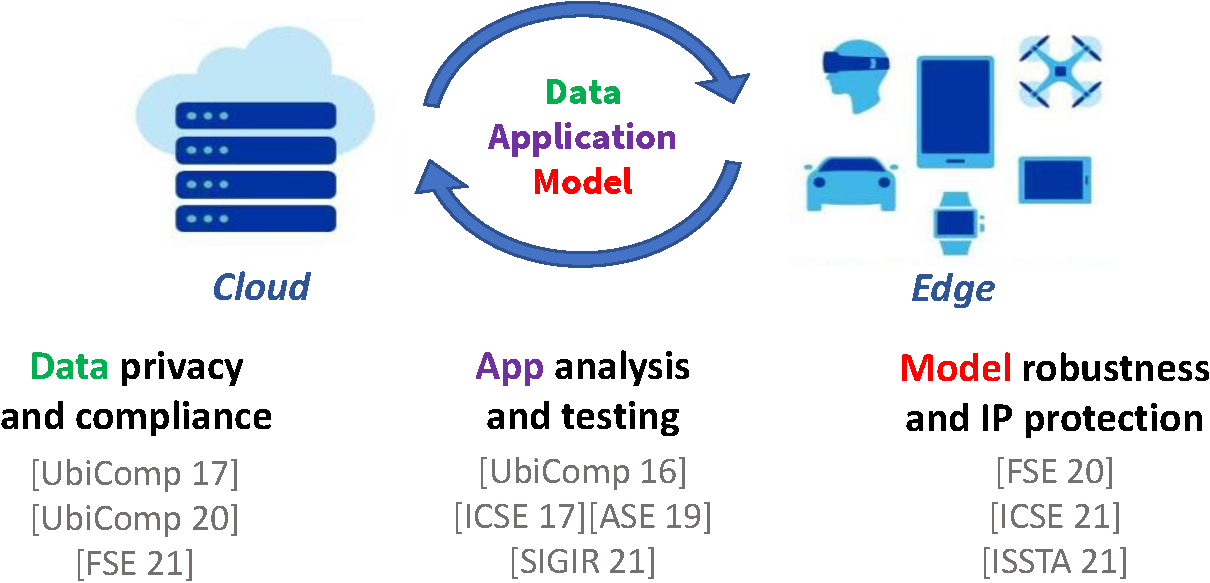
\includegraphics[width=6in]{figures/research_overview.pdf}
    \caption{研究工作概览}
    \label{fig:overview}
\end{figure}

\section{代表性工作}

\subsection{移动应用图形界面分析与测试}
本人博士期间的研究主要面向移动应用,以软件的图形交互界面为切入点对应用程序的功能和隐私特性进行分析。例如,通过程序静态分析和动态分析相结合的方法提取出应用界面与程序代码间的对应关系,以便于理解和自动判别软件中的隐私数据访问行为是否符合用户认知。同时,通过使用大量软件图形界面进行机器学习,可以自动学习到应用程序的交互模式,从而进一步指导应用程序的自动测试生成和动态分析。代表成果\cite{li2016peruim}发表在普适计算领域CCF-A类会议UbiComp 2016中并获得最佳论文提名奖,其相关联工具DroidBot\cite{li2017droidbot}和Humanoid\cite{li2019humanoid}在开源代码托管平台GitHub获得500多个星标\cite{droidbot:code},为领域内熟知。
 
\subsection{隐私保护的边缘端模型域适应}
目前移动和物联网设备上的模型大多是在云端训练后部署到边缘端。在部署过程中,往往需要针对边缘端的数据分布对模型进行域适应以达到更好的预测效果。而同时,边缘端的数据往往是隐私敏感的,如何在保护边缘端数据隐私的情况下进行模型域适应是个重要的问题。在本工作中,我们提出了一种差分隐私的数据分布估计方法,在边缘端采集中间神经元的统计信息(均值、方差等),并计算随机噪声处理数据使其满足差分隐私。这些带有噪声的神经元统计信息就可以在不泄露边缘端隐私信息的同时表示出数据分布,进而帮助云端进行模型的定制训练。代表成果\cite{liu2020pmc}发表在普适计算领域CCF-A类会议UbiComp 2021中。

\subsection{深度神经网络切片分析技术}
程序切片技术是传统程序分析、调试、测试的重要方法之一,旨在从程序代码中提取出与特定关注对象(如变量、API等)相关的子集(切片)。该工作探索了在神经网络中实现程序切片技术的可行性和可能应用。我们提出一种基于正向和反向数据流分析的方法,给定一组输入和输出,可以提取出在模型决策过程中,对预测结果贡献关键作用的神经元子集。该切片技术可以用来分析和解释神经网络决策逻辑,例如可以通过切片模式的差异检测对抗样本、根据神经元的贡献大小对模型进行剪枝等等。工作成果\cite{zhang2020dynamic}发表在软件工程领域CCF-A类会议FSE 2020中。

\subsection{边缘端神经网络模型后门攻击}
边缘端部署的模型很多被用于安全攸关的场景,例如人脸验证、自动驾驶、安防监控等,因此其安全性和可信性尤为重要。该工作主要关注边缘端模型的后门攻击。与传统基于训练数据投毒或二次训练的后门攻击不同,边缘端部署的模型往往已经经过编译压缩,无法继续训练,同时其输入为物理世界的图片而非可以随意进行像素修改的数字输入。本工作受传统软件中的逆向工程方法启发,提出了一个直接在模型计算图上插入恶意旁路的攻击方法,可以在不需要训练的情况下,向目标模型中插入高效、轻量级的后门逻辑。通过对两万多个真实移动应用的扫描分析,我们成功攻击了52个应用中的模型,其中包括下载量数千万的流行应用和安全攸关的支付、商业、儿童教育类应用。工作成果\cite{li2021deeppayload}发表在软件工程领域CCF-A类会议ICSE 2021中。

\subsection{移动端数据处理及隐私保护}
数据的获取和处理是机器学习的关键步骤,尤其是移动端的数据具有很大的利用价值。而同时,由于移动端数据的高度敏感性,以及如今世界各国严格的隐私保护要求(如GDPR等),保护移动用户的隐私也尤为关键。本工作提出一个移动端隐私数据编程框架,在向开发者提供简单易用的流式编程接口的同时,减少代码数据流的碎片化,并进一步通过静态分析获取数据操作的敏感程度。该成果\cite{li2017privacystreams}发表在普适计算领域CCF-A类会议UbiComp 2017中,其对应工具在GitHub获得200多个星标\cite{privacystreams:code},并受多家媒体报道。


\section{未来科研计划}

\subsection{基于移动端分布式机器学习的群体智能研究}
如何理解自然界中的群体智能以及实现人工群体智能是我个人非常感兴趣的研究问题,移动设备丰富的传感能力和逐渐增强的计算能力为群体智能的发展提供了前所未有的机遇。受普适计算领域的众包、群智感知等概念的启发,我希望进一步研究如何让移动个体之间共享知识、共同学习,从而处理更大规模的感知和决策问题,例如如何让家庭和工厂中的智能设备自动协调合作、如何利用泛在的移动设备自动感知城市和环境的状态等等。这其中涉及到系统的搭建、大规模学习节点的性能、容错性,以及节点之间的隐私性等问题亟待解决。

\subsection{软件交互界面的语义理解}
作为之前研究工作的延续,我计划继续以软件交互界面为切入点进行智能软件工程相关的研究。尤其是如今计算机视觉和自然语言处理技术蓬勃发展,为软件交互界面语义理解带来了新的机遇。作为一个多模态的数据类型,对软件交互界面的分析需要同时考虑文本、图像、代码等信息,具有独特的挑战。同时,交互界面的语义理解可以赋能各种新型软件工程任务,例如自动测试、软件无障碍化、机器流程自动化(RPA)等。

\section{教学经历}

在攻读博士期间,我曾多次作为助教,协助导师参与各项教学活动。

\section{预计讲授课程}

\subsection{《智能软件工程》}
卡内基梅隆大学开设有两门与智能软件工程相关的课程,分别是AI4SE\cite{cmu:ai4se}和SE4AI\cite{cmu:se4ai},分别讲解如何用AI技术解决软件工程中的经典问题(如代码分析、需求分析、测试等)和如何用软件分析技术解决AI模型相关的重要问题(例如模型鲁棒性测试和验证、决策过程分析与解释、模型调试等)。我对这两个方向都较为熟悉,可以讲授相关课程。

\subsection{《人工智能的安全、隐私与伦理》}
神经网络的安全隐私及伦理问题是如今热门的研究方向之一,已有很多大学开设了相关课程\cite{ucb:trustworthy,ucb:fairness}。我在微软亚洲研究院开源课程《人工智能系统》\cite{microsoft:ai-system}中担任安全与隐私章节的讲师,也对该方向做过调研和整理,可以讲授相关课程。


{
\bibliographystyle{ieee_fullname}
\bibliography{lyc}
}


\end{document}
